% ═══════════════════════════════════════════════════════════════
% PhD Presentation — PID Activation Steering for Symbolic Music
% ═══════════════════════════════════════════════════════════════
\documentclass[aspectratio=169, 11pt]{beamer}

\usetheme{Madrid}
\usecolortheme{default}

% Clean modern look
\setbeamertemplate{navigation symbols}{}
\setbeamertemplate{footline}{%
  \leavevmode%
  \hbox{%
    \begin{beamercolorbox}[wd=.333333\paperwidth,ht=2.25ex,dp=1ex,center]{author in head/foot}%
      \usebeamerfont{author in head/foot}\insertshortauthor
    \end{beamercolorbox}%
    \begin{beamercolorbox}[wd=.333333\paperwidth,ht=2.25ex,dp=1ex,center]{title in head/foot}%
      \usebeamerfont{title in head/foot}\insertshorttitle
    \end{beamercolorbox}%
    \begin{beamercolorbox}[wd=.333333\paperwidth,ht=2.25ex,dp=1ex,right]{date in head/foot}%
      \usebeamerfont{date in head/foot}\insertframenumber{} / \inserttotalframenumber\hspace*{2ex}
    \end{beamercolorbox}}%
  \vskip0pt%
}

\usepackage{amsmath, amssymb, mathtools}
\usepackage{booktabs}
\usepackage{multirow}
\usepackage{graphicx}
\usepackage{tikz}
\usetikzlibrary{shapes, arrows.meta, positioning, calc, fit, backgrounds}
\usepackage{xcolor}
\usepackage{appendixnumberbeamer}

% Custom colors
\definecolor{pidblue}{RGB}{31, 119, 180}
\definecolor{staticorange}{RGB}{255, 127, 14}
\definecolor{basegreen}{RGB}{44, 160, 44}
\definecolor{alertred}{RGB}{214, 39, 40}
\definecolor{lightgray}{RGB}{240, 240, 240}

\setbeamercolor{block title}{bg=pidblue!20, fg=pidblue!80!black}
\setbeamercolor{block body}{bg=pidblue!5}
\setbeamercolor{block title alerted}{bg=alertred!20, fg=alertred!80!black}
\setbeamercolor{block body alerted}{bg=alertred!5}
\setbeamercolor{block title example}{bg=basegreen!20, fg=basegreen!80!black}
\setbeamercolor{block body example}{bg=basegreen!5}

\title[PID Steering for Music]{Closing the Loop:\\PID Feedback Control for Activation Steering\\in Symbolic Music Generation}
\subtitle{ICML 2026 --- Learning to Listen Workshop}
\author[I. Prokopiou]{Ioannis Prokopiou\inst{1,2} \and Pantelis Vikatos\inst{2} \and Maximos Kaliakatsos-Papakostas\inst{3} \\ \and Theodoros Giannakopoulos\inst{4} \and Themos Stafylakis\inst{1,5}}
\institute[AUEB]{
  \inst{1}Athens University of Economics and Business \and
  \inst{2}Orfium Research \and
  \inst{3}Hellenic Mediterranean University \and
  \inst{4}NCSR ``Demokritos'' \and
  \inst{5}Archimedes / Athena Research Center
}
\date{May 2025}

\begin{document}

% ═══════════════════════════════════════════════════════════════
% TITLE
% ═══════════════════════════════════════════════════════════════
\begin{frame}
\titlepage
\end{frame}

% ═══════════════════════════════════════════════════════════════
% OUTLINE
% ═══════════════════════════════════════════════════════════════
\begin{frame}{Outline}
\tableofcontents
\end{frame}

% ═══════════════════════════════════════════════════════════════
% SECTION 1: MOTIVATION
% ═══════════════════════════════════════════════════════════════
\section{Motivation \& Problem Statement}

\begin{frame}{Why Controllable Music Generation?}

\begin{columns}[T]
\begin{column}{0.55\textwidth}
\textbf{Goal:} Steer a pretrained music model's outputs \emph{at inference time}---no retraining, no fine-tuning.

\vspace{0.5em}
\textbf{Why?}
\begin{itemize}
  \item Retraining is expensive and can degrade unrelated capabilities
  \item Composers need \emph{real-time} creative control (``make it higher-pitched'', ``longer notes'')
  \item Activation steering is lightweight and modular
\end{itemize}

\vspace{0.5em}
\textbf{Our testbed:}
\begin{itemize}
  \item \textbf{Multitrack Music Transformer (MMT)} --- 6-block decoder-only transformer, 12 sublayers, 512-dim, 8 heads
  \item Pre-trained on the Symbolic Orchestral Database (SOD)
  \item Compact 6-tuple MIDI representation: (type, beat, position, pitch, duration, instrument)
\end{itemize}
\end{column}

\begin{column}{0.42\textwidth}
\begin{block}{The Two Papers}
\small
\textbf{ISMIR 2026} (submitted):\\
Dense vs Sparse Activation Steering --- comprehensive comparison, smooth steering envelopes, FMD + human eval

\vspace{0.4em}
\textbf{ICML 2026 Workshop} (this talk):\\
PID feedback control to solve the sparse steering failure mode $\to$ \emph{this presentation}
\end{block}

\vspace{0.3em}
\begin{alertblock}{Key Question}
\small
Can we use \textbf{control theory} to make sparse activation steering smooth and efficient?
\end{alertblock}
\end{column}
\end{columns}

% SPEAKER NOTES:
% - Start by framing the big picture: we want to control what a music AI generates without retraining
% - The MMT is our model: a Transformer that generates polyphonic MIDI
% - We have two papers: the ISMIR paper is the comprehensive comparison, and this ICML workshop paper
%   focuses specifically on the PID control contribution
% - The key question drives the entire paper
\end{frame}

% ═══════════════════════════════════════════════════════════════
\begin{frame}{Background: How Activation Steering Works}

\begin{columns}[T]
\begin{column}{0.48\textwidth}
\textbf{Linear Representation Hypothesis:}\\
Concepts $\approx$ linear directions in activation space.

\vspace{0.5em}
\textbf{Dense Steering (DiffMean):}
\begin{itemize}
  \item Compute centroid difference between ``high pitch'' and ``low pitch'' activation sets
  \item Inject $\mathbf{h}^{(\ell)} \leftarrow \mathbf{h}^{(\ell)} + \alpha \cdot \mathbf{v}^{(\ell)}$ at \emph{every} layer
  \item Problem: pitch \& duration vectors have cosine similarity up to \textbf{0.81} $\to$ feature entanglement
\end{itemize}
\end{column}

\begin{column}{0.48\textwidth}
\textbf{Sparse Activation Steering (SAS):}
\begin{itemize}
  \item Train SAEs: $512 \to 4096$ ($8\times$ expansion)
  \item Top-K sparsity: only $K{=}128$ features active
  \item Monosemantic features $\to$ no entanglement
  \item Single-layer intervention (Layer 10)
  \item 48$\times$ less intervention footprint
\end{itemize}

\vspace{0.3em}
\textbf{Steered activation:}
$$\tilde{\mathbf{a}}_t^\ell = \hat{\mathbf{a}}^\ell\!\Big(\sigma\!\big(f(\mathbf{a}_t^\ell) + \lambda \cdot \mathbf{v}\big)\Big) + \Delta$$

\vspace{0.2em}
{\footnotesize $\sigma$ = Top-K ReLU, $\hat{\mathbf{a}}^\ell$ = SAE decoder, $\Delta$ = reconstruction correction}
\end{column}
\end{columns}

% SPEAKER NOTES:
% - The Linear Representation Hypothesis is the foundation: concepts are directions in the model's latent space
% - Dense steering: take the difference of centroids between two contrastive sets and add it to the residual stream
% - The problem in music: pitch and duration are entangled (0.81 cosine similarity!)
% - SAS solves this: SAEs project to a sparse space where features are monosemantic
% - But SAS introduces a new problem, which is the core of this paper...
\end{frame}

% ═══════════════════════════════════════════════════════════════
\begin{frame}{The Top-K Threshold Problem}

\begin{columns}[T]
\begin{column}{0.48\textwidth}
\begin{alertblock}{The Failure Mode}
When trying to \emph{smoothly} ramp $\lambda$ from 0 to target:
\begin{enumerate}
  \item Fractional $\lambda$ produces small feature additions
  \item These are \textbf{below} the Top-K threshold
  \item Top-K re-sparsification \textbf{zeros them entirely}
  \item Steering signal is \textbf{all-or-nothing}!
\end{enumerate}
\end{alertblock}

\vspace{0.3em}
This is \emph{unique} to sparse steering:
\begin{itemize}
  \item Dense methods: attenuated signals still persist
  \item Sparse methods: sub-threshold $=$ zero
\end{itemize}

\vspace{0.3em}
\textbf{Result:} Instead of a smooth musical transition, you get a \emph{binary jump} --- jarring and unmusical.
\end{column}

\begin{column}{0.48\textwidth}
% FIGURE: topk_threshold_figure_average_duration
% This is Figure 1 from the paper
\begin{center}
\fbox{\parbox{0.9\textwidth}{\centering\vspace{2em}
\textbf{[Figure: Top-K Threshold Failure]}\\[0.5em]
\footnotesize
\textit{Top:} Static cosine ramp vs.\ PID's $\lambda(t)$\\
\textit{Bottom:} Static zeros features during ramp;\\
PID maintains non-zero activations from onset\\[0.5em]
\texttt{figs/topk\_threshold\_figure\_average\_duration}
\vspace{2em}}}
\end{center}

\vspace{0.3em}
\begin{exampleblock}{Key Insight}
\small
We need a controller that can \textbf{push $\lambda$ high enough} to breach the threshold, then \textbf{settle back down} to avoid over-steering.
\end{exampleblock}
\end{column}
\end{columns}

% SPEAKER NOTES:
% - This is the CORE PROBLEM of the paper
% - Walk through the failure mode step by step:
%   1. You want to smoothly ramp steering from 0 to some target
%   2. But the Top-K gate is binary: either your features are in the top 128 or they're zeroed
%   3. Small lambda means small additions, which don't survive the Top-K gate
%   4. So you get NOTHING until lambda is large enough, then suddenly EVERYTHING
% - The figure shows this clearly: static cosine ramp produces zero feature activations throughout the ramp
% - This is qualitatively different from dense steering where any signal, however small, propagates
% - The insight: we need closed-loop control to push past the threshold adaptively
\end{frame}

% ═══════════════════════════════════════════════════════════════
\section{Background: PID Control Theory}

\begin{frame}{PID Control: A 100-Year-Old Solution}

\begin{columns}[T]
\begin{column}{0.55\textwidth}

\textbf{Classical PID controller:}
$$u(t) = \underbrace{K_p \, e(t)}_{\text{Proportional}} + \underbrace{K_i \!\int_0^t\! e(\tau)\,d\tau}_{\text{Integral}} + \underbrace{K_d \,\frac{de(t)}{dt}}_{\text{Derivative}}$$

\vspace{0.3em}
\begin{itemize}
  \item \textbf{P:} Responds to current error. Cannot eliminate steady-state offset.
  \item \textbf{I:} Accumulates past errors $\to$ removes residual bias. \emph{Essential for our problem!}
  \item \textbf{D:} Responds to rate of change $\to$ damps overshoot.
\end{itemize}

\vspace{0.5em}
\textbf{Nguyen et al.\ (ICLR 2026):}\\
Proved that existing steering methods $=$ \textbf{P-only controllers} $\to$ guaranteed steady-state error.
\end{column}

\begin{column}{0.42\textwidth}
% PID Block Diagram
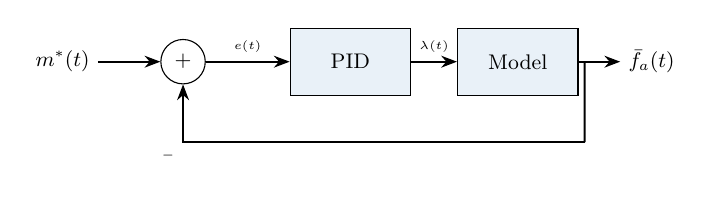
\begin{tikzpicture}[
  block/.style={rectangle, draw, minimum height=1cm, minimum width=1.8cm, fill=pidblue!10, font=\small},
  sum/.style={circle, draw, minimum size=0.5cm, fill=white},
  arr/.style={-{Stealth[length=2mm]}, thick},
  font=\small,
  scale=0.85, transform shape
]
  \node[sum] (sum) at (0,0) {$+$};
  \node[block] (pid) at (2.5,0) {PID};
  \node[block] (plant) at (5,0) {Model};
  \node (input) at (-1.8,0) {$m^*(t)$};
  \node (output) at (7,0) {$\bar{f}_a(t)$};

  \draw[arr] (input) -- (sum);
  \draw[arr] (sum) -- node[above]{\tiny $e(t)$} (pid);
  \draw[arr] (pid) -- node[above]{\tiny $\lambda(t)$} (plant);
  \draw[arr] (plant) -- (output);

  % Feedback
  \coordinate (fb) at (6, -1.2);
  \draw[thick] (6,0) -- (fb);
  \draw[arr] (fb) -| node[below left]{\tiny $-$} (sum);
\end{tikzpicture}

\vspace{0.5em}
\begin{block}{Our Translation}
\small
\begin{tabular}{ll}
Setpoint & $m^*(t)$: target activation \\
Output & $\bar{f}_a(t)$: measured features \\
Control & $\lambda(t)$: steering magnitude \\
Plant & MMT + SAE at Layer 10 \\
\end{tabular}
\end{block}
\end{column}
\end{columns}

% SPEAKER NOTES:
% - PID control has been used since the 1920s --- it's one of the most widely deployed algorithms ever
% - The key insight from Nguyen et al. (ICLR 2026): existing activation steering is just P-control
%   - They proved this mathematically by modeling the layer-wise forward pass as a dynamical system
%   - P-only = guaranteed steady-state error from model priors
% - The I term is what we need: it accumulates error over time, which will push lambda past the threshold
% - The D term helps with stability at the transition point
% - The block diagram shows how we translate this to our setting:
%   - Setpoint: what we want the feature activations to be
%   - Output: what the features actually are after Top-K
%   - Control signal: lambda(t), the steering magnitude
%   - Plant: the model itself
\end{frame}

% ═══════════════════════════════════════════════════════════════
\section{Method}

\begin{frame}{Two Forms of PID Steering}

\begin{columns}[T]
\begin{column}{0.48\textwidth}
\begin{block}{\textbf{Spatial PID} (Layer-wise)}
\vspace{0.3em}
Adapts Nguyen et al.\ to the MMT.

$$\mathbf{u}(k) = K_p \mathbf{e}(k) + K_i \!\!\sum_{j=0}^{k-1}\!\mathbf{e}(j) + K_d \Delta\mathbf{e}(k)$$

\begin{itemize}
  \item DiffMean vectors across 12 sublayers
  \item All-to-all injection (sequential)
  \item Challenge: only 12 layers (vs.\ 32+ in LLMs) $\to$ fewer steps for I-term
  \item $\Rightarrow$ Requires $8\times$ higher $K_i$ for pitch vs.\ duration
\end{itemize}

\vspace{0.2em}
\textbf{Purpose:} Domain validation --- replicates control-theoretic predictions in music.
\end{block}
\end{column}

\begin{column}{0.48\textwidth}
\begin{block}{\textbf{Temporal PID} (Step-wise) \hfill {\color{alertred}$\star$ Main Contribution}}
\vspace{0.3em}
Transposes PID to the autoregressive \emph{time} axis.

$$\lambda(t) = \text{clamp}\!\Big(K_p e(t) + K_i I(t\!-\!1) + K_d \Delta e(t)\Big)$$

\begin{itemize}
  \item SAS at single layer (Layer 10) $\to$ \textbf{cannot} do spatial PID
  \item Controller adjusts $\lambda$ at \emph{each generation step}
  \item Closed-loop: measures whether features survived Top-K
  \item Anti-windup clamping: $I \in [-I_\text{max}, I_\text{max}]$
\end{itemize}

\vspace{0.2em}
\textbf{Purpose:} Solve the Top-K threshold problem for sparse steering.
\end{block}
\end{column}
\end{columns}

% SPEAKER NOTES:
% - We have TWO forms of PID, serving different purposes
% - Spatial PID is the more straightforward adaptation: apply PID across layers, just like Nguyen et al.
%   - But the MMT only has 12 layers vs 32+ in LLMs, so the I-term has fewer steps
%   - Interesting finding: pitch needs 8x higher Ki than duration (model's autoregressive priors resist pitch changes)
%   - This primarily serves as domain validation
% - Temporal PID is the MAIN CONTRIBUTION:
%   - SAS operates at a single layer, so spatial PID is impossible
%   - Instead, we control lambda over TIME (generation steps)
%   - At each token, we measure the features, compute error, adjust lambda
%   - This is a fundamentally new way to apply PID control to steering
\end{frame}

% ═══════════════════════════════════════════════════════════════
\begin{frame}{Temporal PID: The Mechanism}

\begin{columns}[T]
\begin{column}{0.52\textwidth}
\textbf{Step 1: Measure} --- ``Concept Fingerprint''
$$\bar{f}_a(t) = \frac{1}{|\mathcal{T}|} \sum_{j \in \mathcal{T}} f(\mathbf{a}_t^\ell)_j$$
{\small Top $N{=}32$ features by $|v_j|$ --- did they survive Top-K?}

\vspace{0.4em}
\textbf{Step 2: Compute error}
$$e(t) = m^*(t) - \bar{f}_a(t)$$
{\small Setpoint $m^*(t)$: cosine ramp over $T_\text{ramp}$ beats}

\vspace{0.4em}
\textbf{Step 3: Update $\lambda(t)$}
$$\lambda(t) = \text{clamp}\Big(K_p e(t) + K_i I(t{-}1) + K_d \Delta e\Big)$$

\vspace{0.4em}
\textbf{Step 4: Steer \& re-sparsify}
$$\mathbf{s}(t) = f(\mathbf{a}_t^\ell) + \lambda(t) \cdot \mathbf{v} \quad\to\quad \text{Top-K}(\mathbf{s}(t))$$
\end{column}

\begin{column}{0.44\textwidth}
\begin{exampleblock}{How the I-term solves it}
\small
\begin{enumerate}
  \item Ramp begins: $\bar{f}_a \approx 0$ (features below threshold)
  \item Error $e(t) > 0$ persists
  \item I-term \textbf{accumulates}: $I(t) = I(t{-}1) + e(t)$
  \item $\lambda(t)$ grows progressively
  \item Eventually $\lambda$ is \textbf{large enough} to breach Top-K
  \item Features activate! Error drops.
  \item Controller \textbf{settles} to minimal $\lambda$
  \item D-term damps overshoot at transition
\end{enumerate}
\end{exampleblock}

\vspace{0.3em}
\begin{block}{Hyperparameters}
\small
\begin{tabular}{ll}
$K_p = 1.0$ & $K_d = 0.01$ \\
$K_i$: pitch $= 0.05$ & $K_i$: dur $= 0.025$ \\
$I_\text{max} = 10$ & $\lambda_\text{max} = 3.0$ \\
$T_\text{ramp} = 64$ & $N = 32$ features \\
\end{tabular}
\end{block}
\end{column}
\end{columns}

% SPEAKER NOTES:
% - Walk through the 4 steps at each generation step:
%   1. MEASURE: We look at the 32 most important features and check their activations
%      - This is the "concept fingerprint" - tells us if our steering signal survived the Top-K gate
%   2. ERROR: Compare to what we want (cosine-ramped setpoint)
%   3. UPDATE: PID control law computes lambda - note the anti-windup clamping on I
%   4. STEER: Add lambda * v to the sparse representation, then re-sparsify
% - The I-term is the hero: when features are zeroed, error accumulates, pushing lambda up
%   until it breaches the threshold, then it settles back down
% - Note the 8x Ki asymmetry: pitch = 0.05, duration = 0.025
%   - This comes from the spatial PID grid search
%   - Pitch has stronger autoregressive priors (the model really resists changing pitch register)
\end{frame}

% ═══════════════════════════════════════════════════════════════
\section{Experiments \& Results}

\begin{frame}{Experimental Setup}

\begin{columns}[T]
\begin{column}{0.48\textwidth}
\textbf{Model \& Data:}
\begin{itemize}
  \item MMT pre-trained on SOD (4,474 pieces)
  \item Ground truth: $H_0{=}2.974$, $S_0{=}92.3\%$, $G_0{=}93.1\%$
  \item Contrastive sets: 1,280 samples each
  \item Pitch: $\leq$60 vs.\ $\geq$67.6 semitones
  \item Duration: $\leq$6.5 vs.\ $\geq$14.5 ticks
\end{itemize}

\vspace{0.5em}
\textbf{SAE Architecture:}
\begin{itemize}
  \item One per layer: $512 \to 4096$ ($8\times$)
  \item Top-K with $K{=}128$ (Layer 10)
  \item Trained on 640K activation vectors
\end{itemize}
\end{column}

\begin{column}{0.48\textwidth}
\textbf{Quality Metric:}
$$\delta = |H - H_0| + \max(0, S_0 - S) + \max(0, G_0 - G)$$
{\small Asymmetric: penalizes only \emph{decreases} in scale/groove consistency}

\vspace{0.5em}
\textbf{FMD:}
\begin{itemize}
  \item CLaMP2 embeddings (512-dim)
  \item MLE Gaussian estimation
  \item Reference: 4,474 SOD MIDIs
\end{itemize}

\vspace{0.5em}
\textbf{Generation:}
\begin{itemize}
  \item Temperature 1.0, top-$k$ logit filtering (0.9)
  \item max\_seq\_len = 1024
  \item $n{=}40$ samples per condition
\end{itemize}
\end{column}
\end{columns}

% SPEAKER NOTES:
% - Quick setup overview --- the important things to note:
%   - We use contrastive sets from the 20th/80th percentiles of the training data
%   - The quality metric delta is a composite: entropy + scale consistency + groove consistency
%     - Asymmetric: we don't penalize increases in scale/groove (those are benign)
%   - FMD measures distributional distance from the reference corpus (like FID for images)
%   - All numbers are from 40 generations per condition with bootstrap CIs
\end{frame}

% ═══════════════════════════════════════════════════════════════
\begin{frame}{Result 1: Spatial PID Validates Control Theory in Music}

\begin{columns}[T]
\begin{column}{0.48\textwidth}
\textbf{Grid search} (150 configs per concept):

\vspace{0.3em}
\begin{table}
\centering\small
\begin{tabular}{lccc}
  \toprule
  Concept & $K_p$ & $K_i$ & $K_d$ \\
  \midrule
  Pitch & 1.5 & \textbf{0.2} & 0.01 \\
  Duration & 1.25 & \textbf{0.025} & 0.01 \\
  \bottomrule
\end{tabular}
\end{table}

\begin{alertblock}{$8\times$ $K_i$ Asymmetry}
\small
Pitch requires $8\times$ more integral gain than duration. The model's autoregressive priors strongly resist pitch register changes.
\end{alertblock}
\end{column}

\begin{column}{0.48\textwidth}
\textbf{Key findings:}

\begin{itemize}
  \item PI/PID eliminate P-control's residual error within 12 layers $\to$ replicates Nguyen et al.
  \item PID reduces $\delta$ by \textbf{17--47\%} vs.\ P-only across 9 hook configurations
  \item All-12 sublayers is optimal injection strategy
  \item Single-layer PID shows \textbf{47\% $\delta$ reduction} at Layer 10
\end{itemize}

\vspace{0.3em}
\begin{exampleblock}{Takeaway}
\small
Control-theoretic predictions hold even in a \emph{shallow} music Transformer. The $8\times$ $K_i$ asymmetry is a domain-specific discovery.
\end{exampleblock}
\end{column}
\end{columns}

% SPEAKER NOTES:
% - Spatial PID is the validation study
% - The main finding is the 8x Ki asymmetry between pitch and duration
%   - This is a genuine discovery about the MMT: pitch has much stronger priors
%   - We hypothesize this reflects "pitch anchoring" — the model really wants to stay in a register
%   - Duration is more malleable
% - We replicate Nguyen et al.'s theoretical predictions: I-term eliminates steady-state error
% - PID helps most at concentrated injection points (Layer 10: 47% delta reduction)
% - This motivates the temporal PID: if PID helps this much in dense space, what about sparse?
\end{frame}

% ═══════════════════════════════════════════════════════════════
\begin{frame}{Result 2: Temporal PID --- Single-Concept Steering}

\begin{columns}[T]
\begin{column}{0.52\textwidth}
\begin{table}
\centering\small
\caption*{\textbf{Single-concept results} ($n{=}40$, $\lambda_\text{max}{=}3.0$)}
\begin{tabular}{llccc}
  \toprule
  Concept & Dir. & \textbf{PID} & Static & Base \\
  \midrule
  \multirow{2}{*}{Pitch (st)} & $\uparrow$ & \textbf{72.65} & 72.30 & 68.79 \\
  & $\downarrow$ & \textbf{43.99} & 44.91 & 67.94 \\
  \multirow{2}{*}{Dur.\ (ticks)} & $\uparrow$ & \textbf{18.87} & 22.17 & 7.99 \\
  & $\downarrow$ & 4.23 & \textbf{3.35} & 7.72 \\
  \midrule
  \multicolumn{2}{l}{Pitch FMD} & \textbf{461.9} & 487.7 & 381.5 \\
  \multicolumn{2}{l}{Dur.\ FMD} & \textbf{501.2} & 525.9 & 385.3 \\
  \bottomrule
\end{tabular}
\end{table}

\vspace{0.2em}
\small
\textbf{Pitch up:} PID $\delta{=}0.45$ vs.\ Static $\delta{=}0.64$\\
\textbf{FMD:} PID 5.3\% lower (drift--control tradeoff)
\end{column}

\begin{column}{0.44\textwidth}
\textbf{Headline numbers:}

\vspace{0.3em}
\begin{block}{Intervention Efficiency}
\centering\large
\textbf{62\% less $\lambda$}\\[0.2em]
\small avg $\lambda{=}1.15$ vs.\ static $\lambda{=}3.0$\\[0.3em]
\large \textbf{5\% lower FMD}\\[0.2em]
\small for pitch steering
\end{block}

\vspace{0.3em}
\begin{block}{Smoothness}
\small
$\text{std}(\Delta\bar{f}_a) < 0.003$ per step\\
vs.\ static: \textbf{binary jump}
\end{block}

\vspace{0.3em}
{\footnotesize\color{gray} CIs: $\delta_\text{PID} = 0.45$ [0.33, 0.62] vs.\\ $\delta_\text{Static} = 0.64$ [0.47, 0.85]}
\end{column}
\end{columns}

% SPEAKER NOTES:
% - This is the MAIN RESULTS slide
% - PID matches or exceeds static SAS in steering effectiveness for pitch
% - But the key advantage is EFFICIENCY: avg lambda = 1.15 vs 3.0 (62% less intervention!)
%   - The controller finds the minimum lambda needed to sustain the steering
% - FMD is 5% lower: dynamic lambda avoids over-steering early tokens
%   - This is a drift-control tradeoff: any steering increases FMD, PID minimizes the drift
% - Smoothness: feature activations change by <0.003 per step vs binary jump for static
% - Duration-up is the exception (we'll discuss this later)
% - Note: static SAS at lambda=3.0 is the standard approach — it uses the max, like a sledgehammer
\end{frame}

% ═══════════════════════════════════════════════════════════════
\begin{frame}{Result 3: $\lambda(t)$ Trajectory \& Component Ablation}

\begin{columns}[T]
\begin{column}{0.48\textwidth}
% FIGURE: hero_lambda_trajectories.png
% This is Figure 2 from the paper
\begin{center}
\fbox{\parbox{0.9\textwidth}{\centering\vspace{2.5em}
\textbf{[Figure: PID $\lambda(t)$ Trajectory]}\\[0.5em]
\footnotesize
Pitch-up, $m_\text{target}{=}2.0$\\
Controller overshoots briefly at threshold breach,\\
then settles to $\lambda \approx 1.15$\\
(62\% below static's $\lambda{=}3.0$)\\[0.5em]
\texttt{figs/hero\_lambda\_trajectories.png}
\vspace{2.5em}}}
\end{center}

\vspace{0.2em}
{\small The trajectory shows classic PID behavior: ramp-up, brief overshoot, then steady-state settling.}
\end{column}

\begin{column}{0.48\textwidth}
\textbf{Component Ablation:}

\vspace{0.3em}
\begin{table}
\centering\small
\begin{tabular}{lcc}
  \toprule
  Controller & avg $\lambda$ & Breaches threshold? \\
  \midrule
  P-only & 0.664 & \color{alertred}\textbf{No} \\
  PI & 1.136 & \color{basegreen}\textbf{Yes} \\
  PID & 1.158 & \color{basegreen}\textbf{Yes} \\
  \bottomrule
\end{tabular}
\end{table}

\vspace{0.3em}
\begin{alertblock}{The I-term is Essential}
\small
P-only: $\lambda_\text{avg}{=}0.664$ --- too conservative, \textbf{never breaches} the Top-K threshold.

\vspace{0.2em}
Adding I: $\lambda_\text{avg}$ jumps to 1.136 --- error accumulation pushes past the threshold.

\vspace{0.2em}
Adding D: marginal settling improvement ($\lambda_\text{avg}{=}1.158$). The slowly-varying cosine setpoint limits D's contribution.
\end{alertblock}
\end{column}
\end{columns}

% SPEAKER NOTES:
% - LEFT: The lambda trajectory is the "hero figure" of the paper
%   - Shows the controller ramping up, overshooting briefly, then settling at ~1.15
%   - Static SAS would be a flat line at 3.0 --- wasteful!
% - RIGHT: The ablation proves that the I-term is the essential ingredient
%   - P-only: lambda = 0.664 on average --- it NEVER breaches the threshold
%   - Adding I: lambda jumps to 1.136 --- error accumulation works!
%   - Adding D: minimal improvement --- the setpoint is slowly varying, so D doesn't have much to work with
%   - This is expected: D matters most for rapid setpoint changes or disturbances
\end{frame}

% ═══════════════════════════════════════════════════════════════
\begin{frame}{Result 4: Dual-Concept Steering}

\begin{columns}[T]
\begin{column}{0.48\textwidth}
Two independent PID controllers, one per concept. Orthogonalized SAS vectors + expanded $2\times K$ budget.

\vspace{0.3em}
\begin{table}
\centering\small
\begin{tabular}{llcc}
  \toprule
  Setting & Method & $\delta\,(\downarrow)$ & Dual\% \\
  \midrule
  \multirow{2}{*}{Uncond.} & PID & \textbf{0.47} & 75\% \\
  & Static & 2.19 & \textbf{95\%} \\
  \midrule
  \multirow{2}{*}{L/L$\to$H/S} & PID & \textbf{2.36} & 80\% \\
  & Static & 2.85 & 85\% \\
  \multirow{2}{*}{H/S$\to$L/L} & PID & \textbf{1.92} & 100\% \\
  & Static & 4.30 & 100\% \\
  \bottomrule
\end{tabular}
\end{table}
\end{column}

\begin{column}{0.48\textwidth}
\textbf{Unconditioned:}
\begin{itemize}
  \item PID: $4.7\times$ lower $\delta$ (0.47 vs.\ 2.19)
  \item But lower dual success (75\% vs.\ 95\%)
  \item PID's conservative $\lambda$ under-steers duration
\end{itemize}

\vspace{0.3em}
\textbf{Hardest case (H/S$\to$L/L):}
\begin{itemize}
  \item Opposing-direction steering on 16-beat prefixes
  \item PID: $2.2\times$ less degradation
  \item Both methods: 100\% success
\end{itemize}

\vspace{0.3em}
\begin{block}{Quality--Success Tradeoff}
\small
PID trades some steering success for much better quality preservation. Higher $m_\text{target}$ or concept-specific setpoints could recover accuracy.
\end{block}
\end{column}
\end{columns}

% SPEAKER NOTES:
% - Dual-concept steering is harder: you need to steer BOTH pitch AND duration simultaneously
% - We use two independent PID controllers with orthogonalized SAS vectors
% - Key finding: PID achieves 4.7x lower quality degradation in unconditioned generation
%   - But at the cost of lower dual success (75% vs 95%)
%   - This is because PID's conservative lambda sometimes doesn't push duration hard enough
%   - Duration is the weaker-responding attribute
% - In the hardest conditioned case (opposing directions), PID really shines:
%   - 100% success with 2.2x less degradation
% - The lambda trajectories are highly correlated (r=0.998) since both respond to same cosine ramp
%   - But magnitudes differ: pitch settles at 1.15, duration at 1.05
%   - The concept-specific Ki provides meaningful calibration
\end{frame}

% ═══════════════════════════════════════════════════════════════
\section{Robustness \& Analysis}

\begin{frame}{Robustness: Gain Sweeps \& $T_\text{ramp}$ Sensitivity}

\begin{columns}[T]
\begin{column}{0.48\textwidth}
\textbf{Gain Robustness} ($2\times$ perturbation range):

\vspace{0.3em}
{\small Swept $K_p, K_i$ at factors $\{0.5, 0.75, 1.0, 1.25, 1.5, 2.0\}$}

\vspace{0.3em}
\begin{exampleblock}{Pitch: Remarkably Stable}
\small
All 12 configurations:\\
Pitch $\in$ [72.77, 75.12] st\\
(range: 2.35 st over $4\times$ gain variation)
\end{exampleblock}

\begin{exampleblock}{Duration: Also Stable}
\small
Duration $\in$ [15.13, 19.85] ticks\\
Even $K_p{=}0.5$ (extreme) still steers meaningfully above baseline (7.99 ticks)
\end{exampleblock}

\vspace{0.2em}
{\small\textbf{Practical implication:} Gains don't need precise tuning. $2\times$ off from optimal still works.}
\end{column}

\begin{column}{0.48\textwidth}
\textbf{$T_\text{ramp}$ Sensitivity:}

\vspace{0.3em}
\begin{table}
\centering\small
\begin{tabular}{cccc}
  \toprule
  $T_\text{ramp}$ & Pitch & $\delta$ & avg $\lambda$ \\
  \midrule
  16 & 70.07 & \color{alertred}10.17 & 1.216 \\
  \textbf{32} & \textbf{73.86} & \textbf{0.82} & 1.162 \\
  \textbf{64} & \textbf{73.56} & \textbf{2.13} & 1.167 \\
  128 & 73.41 & 4.40 & 1.076 \\
  256 & 71.20 & 4.34 & 0.903 \\
  \bottomrule
\end{tabular}
\end{table}

\vspace{0.3em}
\begin{block}{Sweet Spot: $T_\text{ramp} \in \{32, 64\}$}
\small
\textbf{Too short} (16): aggressive I-accumulation $\to$ quality collapse ($\delta{=}10.17$)

\textbf{Too long} (256): delayed I-buildup $\to$ weaker steering, lower $\lambda$
\end{block}
\end{column}
\end{columns}

% SPEAKER NOTES:
% - These robustness experiments were run specifically in response to reviewer requests
% - Gain sweeps: the controller is very robust to gain perturbations
%   - Even 2x off from nominal, pitch still steers to 72-75 st (baseline is 68.79)
%   - This matters for practical deployment: you don't need perfect gain tuning
% - T_ramp sensitivity shows a clear sweet spot at 32 and 64:
%   - Too short = aggressive integral accumulation = quality collapse
%   - Too long = the I term doesn't build up fast enough = weak steering
%   - 64 is our default: good balance of smooth onset and timely convergence
\end{frame}

% ═══════════════════════════════════════════════════════════════
\begin{frame}{Analysis: The Duration-Up Problem}

\begin{columns}[T]
\begin{column}{0.48\textwidth}
\begin{alertblock}{Duration-Up: PID Underperforms}
\small
PID $\delta{=}8.45$ vs.\ Static $\delta{=}2.84$

\vspace{0.2em}
Scale consistency: PID 84.7\% vs.\ Static 92.4\%

\vspace{0.2em}
\textbf{Why?}
\end{alertblock}

\vspace{0.3em}
\textbf{Matched-$\lambda$ experiment:}
\begin{itemize}
  \item Static SAS at $\lambda{=}1.0$ (same as PID's average): scale = 91.3\%
  \item PID at avg $\lambda{\approx}1.0$: scale = 84.7\%
  \item Gap: $6.6$ percentage points
\end{itemize}

\vspace{0.3em}
\textbf{Diagnosis:} PID's \emph{within-sequence} $\lambda$ variation generates tokens at varying steering magnitudes $\to$ creates pitch-duration coupling inconsistencies that a constant $\lambda$ avoids.
\end{column}

\begin{column}{0.48\textwidth}
\begin{table}
\centering\small
\caption*{Static SAS at matched $\lambda$ (duration-up)}
\begin{tabular}{cccc}
  \toprule
  $\lambda$ & Dur. & Scale\% & $\delta$ \\
  \midrule
  0.5 & 12.33 & 95.1 & 1.59 \\
  \textbf{1.0} & \textbf{21.19} & \textbf{91.3} & \textbf{2.89} \\
  1.5 & 22.44 & 93.2 & 1.88 \\
  2.0 & 22.80 & 91.1 & 4.12 \\
  3.0 & 24.41 & 93.7 & 5.80 \\
  \bottomrule
\end{tabular}
\end{table}

\vspace{0.2em}
All static configs maintain scale $\geq 91\%$\\
PID's dynamic trajectory: only 84.7\%

\vspace{0.3em}
\begin{block}{Proposed Fix (Future Work)}
\small
Piecewise-constant $\lambda$: hold $\lambda$ fixed within musical phrases to reduce intra-sequence variation.
\end{block}
\end{column}
\end{columns}

% SPEAKER NOTES:
% - This is the honest limitation slide — duration-up is where PID struggles
% - The matched-lambda experiment was key to understanding WHY:
%   - Static SAS at the same average lambda (1.0) maintains 91.3% scale
%   - PID at average lambda ~1.0 only gets 84.7%
%   - The difference: PID varies lambda WITHIN a sequence (ramp up, then settle)
%   - This variation creates inconsistencies in the generated tokens
%   - Pitch steering doesn't have this problem — pitch is more robust to lambda variation
% - Note: this is attribute-specific. It's about how the duration SAS vector interacts with scale consistency
% - Proposed fix: hold lambda constant within musical phrases (piecewise scheduling)
\end{frame}

% ═══════════════════════════════════════════════════════════════
\begin{frame}{Dense vs.\ Sparse: The Fundamental Tradeoff}

\begin{center}
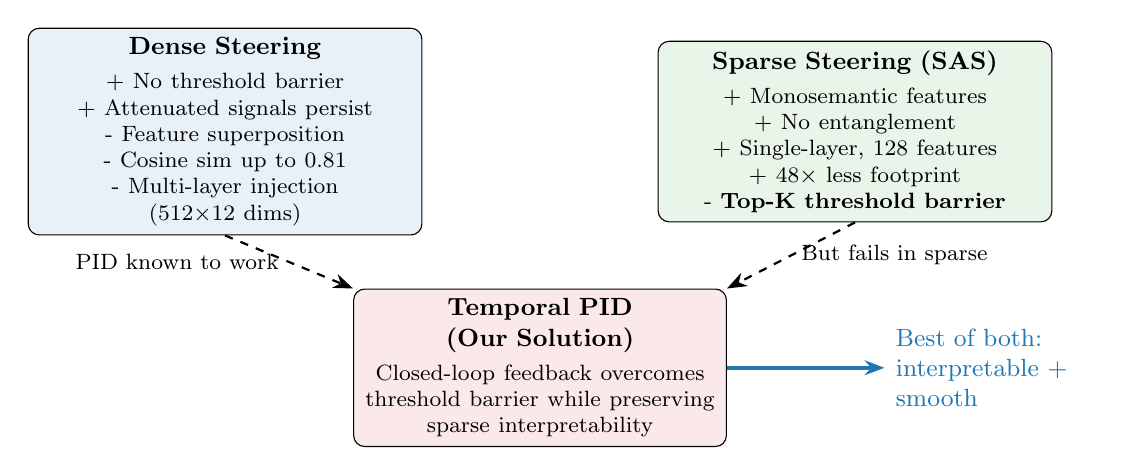
\begin{tikzpicture}[
  block/.style={rectangle, draw, rounded corners, minimum height=2cm, minimum width=5cm, text width=4.5cm, align=center, font=\small},
]
  \node[block, fill=pidblue!10] (dense) at (-4,0) {
    \textbf{Dense Steering}\\[0.3em]
    {\footnotesize
    + No threshold barrier\\
    + Attenuated signals persist\\
    - Feature superposition\\
    - Cosine sim up to 0.81\\
    - Multi-layer injection\\
    (512$\times$12 dims)\\
    }
  };

  \node[block, fill=basegreen!10] (sparse) at (4,0) {
    \textbf{Sparse Steering (SAS)}\\[0.3em]
    {\footnotesize
    + Monosemantic features\\
    + No entanglement\\
    + Single-layer, 128 features\\
    + 48$\times$ less footprint\\
    - \textbf{Top-K threshold barrier}\\
    }
  };

  \node[block, fill=alertred!10, minimum width=4.5cm] (pid) at (0,-3) {
    \textbf{Temporal PID (Our Solution)}\\[0.3em]
    {\footnotesize
    Closed-loop feedback overcomes\\
    threshold barrier while preserving\\
    sparse interpretability\\
    }
  };

  \draw[-{Stealth[length=2.5mm]}, thick, dashed] (dense.south) -- (pid.north west) node[midway, left, font=\footnotesize] {PID known to work};
  \draw[-{Stealth[length=2.5mm]}, thick, dashed] (sparse.south) -- (pid.north east) node[midway, right, font=\footnotesize] {But fails in sparse};
  \draw[-{Stealth[length=2.5mm]}, ultra thick, pidblue] (pid.east) -- ++(2,0) node[right, font=\small, text width=2.5cm] {Best of both:\\interpretable +\\smooth};
\end{tikzpicture}
\end{center}

% SPEAKER NOTES:
% - This diagram captures the conceptual contribution
% - Dense steering: works well with PID (Nguyen et al proved this), but suffers from entanglement
% - Sparse steering: solves entanglement but introduces the Top-K threshold barrier
% - Our contribution: temporal PID gives you the best of both worlds
%   - You keep the interpretability and monosemanticity of sparse features
%   - But you overcome the threshold barrier through closed-loop feedback
% - The key novelty is NOT PID itself (that's classical), but the temporal closed-loop feedback system
%   built around a Top-K-aware error signal
\end{frame}

% ═══════════════════════════════════════════════════════════════
\section{Limitations \& Future Work}

\begin{frame}{Limitations \& Future Directions}

\begin{columns}[T]
\begin{column}{0.48\textwidth}
\textbf{Current Limitations:}
\begin{itemize}
  \item Single model (MMT) and dataset (SOD)
  \item $8\times$ $K_i$ asymmetry may be model-specific
  \item Duration-up degrades scale consistency
  \item Sample sizes ($n{=}40$) --- modest
  \item No perceptual (human) evaluation in this paper
  \item D-term not formally ablated (PID vs.\ PI)
  \item Average $\lambda$ is a proxy for intervention footprint
\end{itemize}

\vspace{0.5em}
\textbf{What the reviewers said:}\\
{\small ``I think it should be accepted [...] a temporal closed-loop built around a Top-K-aware error signal; making that distinction even sharper would help.''}
\end{column}

\begin{column}{0.48\textwidth}
\textbf{Future Work:}
\begin{enumerate}
  \item \textbf{Cross-architecture validation}\\
    {\small Test on larger models, different music domains}
  \item \textbf{Adaptive gain scheduling}\\
    {\small Learn $K_i$ per-concept automatically}
  \item \textbf{Piecewise-constant $\lambda$}\\
    {\small Fix the duration-up problem}
  \item \textbf{Soft Top-K alternatives}\\
    {\small JumpReLU SAEs could smooth the barrier}
  \item \textbf{Direct intervention metrics}\\
    {\small $|\Delta\text{TopK}|$ or $L_1$ norm instead of avg $\lambda$}
  \item \textbf{Perceptual evaluation}\\
    {\small Human listening studies (in ISMIR paper)}
  \item \textbf{Plausibility-gated methods}\\
    {\small DIRECTER-style rejection for OOD safety}
\end{enumerate}
\end{column}
\end{columns}

% SPEAKER NOTES:
% - Be honest about limitations:
%   - Single model/dataset is the biggest one — we don't know if the 8x Ki asymmetry is universal
%   - Duration-up is a genuine failure mode that needs work
%   - No human evaluation in this workshop paper (but the ISMIR paper has it)
% - The reviewer feedback was positive — recommended acceptance
%   - Key suggestion: sharpen the novelty claim (temporal closed-loop, not PID per se)
%   - We addressed this and several other suggestions
% - Future work is exciting:
%   - JumpReLU SAEs could eliminate the threshold problem entirely (no hard Top-K gate)
%   - Adaptive gain scheduling would remove the need for manual Ki tuning
%   - Piecewise-constant lambda could fix duration-up
\end{frame}

% ═══════════════════════════════════════════════════════════════
\section{Summary}

\begin{frame}{Key Takeaways}

\begin{columns}[T]
\begin{column}{0.55\textwidth}

\begin{enumerate}
  \item[\color{pidblue}\textbf{1.}] \textbf{Identified a fundamental failure mode} in sparse activation steering: the Top-K threshold zeroes smooth ramping signals entirely

  \vspace{0.4em}
  \item[\color{pidblue}\textbf{2.}] \textbf{Proposed Temporal PID Steering:} a closed-loop feedback system that measures whether features survive re-sparsification and adapts $\lambda(t)$ accordingly

  \vspace{0.4em}
  \item[\color{pidblue}\textbf{3.}] \textbf{The I-term is essential:} it accumulates error to push $\lambda$ past the threshold, then the controller settles to a minimal intervention

  \vspace{0.4em}
  \item[\color{pidblue}\textbf{4.}] \textbf{Results:} 43--62\% less intervention, 5\% lower FMD, smooth transitions, robust to $2\times$ gain perturbations

  \vspace{0.4em}
  \item[\color{pidblue}\textbf{5.}] \textbf{Domain insight:} Pitch needs $8\times$ more integral gain than duration --- reflects model-specific autoregressive priors
\end{enumerate}
\end{column}

\begin{column}{0.42\textwidth}
\begin{block}{One-Sentence Summary}
\large
We use PID control to make sparse activation steering \textbf{smooth} and \textbf{efficient} in symbolic music generation, by closing the loop around the Top-K sparsity gate.
\end{block}

\vspace{0.5em}
\begin{center}
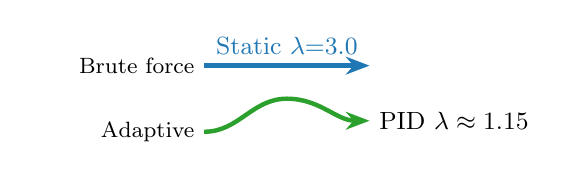
\begin{tikzpicture}[scale=0.7]
  \draw[-{Stealth[length=3mm]}, ultra thick, pidblue] (0,0) -- (3,0) node[midway, above, font=\small] {Static $\lambda{=}3.0$};
  \draw[-{Stealth[length=3mm]}, ultra thick, basegreen] (0,-1.2) to[out=0, in=180] (1.5,-0.6) to[out=0,in=180] (3,-1.0);
  \node[right, font=\small] at (3,-1.0) {PID $\lambda \approx 1.15$};
  \node[left, font=\footnotesize, text width=2cm, align=right] at (0,0) {Brute force};
  \node[left, font=\footnotesize, text width=2cm, align=right] at (0,-1.2) {Adaptive};
\end{tikzpicture}
\end{center}
\end{block}
\end{column}
\end{columns}

% SPEAKER NOTES:
% - Wrap up with the 5 key takeaways
% - 1. We found a real problem: smooth ramping fails completely in sparse steering
% - 2. Our solution: temporal PID control — the first closed-loop feedback for sparse steering
% - 3. The I-term is the hero — without it, lambda never breaches the threshold
% - 4. Numbers: 62% less intervention for pitch, 5% lower FMD, smooth transitions
% - 5. Domain insight: the 8x Ki asymmetry tells us something about how the model represents pitch vs duration
% - One-sentence: close the loop around the Top-K gate
\end{frame}

% ═══════════════════════════════════════════════════════════════
\begin{frame}{}
\begin{center}
\vspace{2em}
{\Huge Thank you!}

\vspace{1.5em}
{\Large Questions?}

\vspace{2em}
{\large Ioannis Prokopiou}\\
{\normalsize gian.prokopiou@aueb.gr}

\vspace{1.5em}
{\small
ICML 2026 --- Learning to Listen Workshop\\[0.3em]
\textit{Closing the Loop: PID Feedback Control for\\Activation Steering in Symbolic Music Generation}
}
\end{center}
\end{frame}

% ═══════════════════════════════════════════════════════════════
% BACKUP / APPENDIX SLIDES
% ═══════════════════════════════════════════════════════════════
\appendix

\begin{frame}[noframenumbering]{Backup: Confidence Intervals}

\begin{table}
\centering\small
\caption*{Bootstrap 95\% CIs ($n{=}40$, 10,000 resamples)}
\begin{tabular}{lccc}
  \toprule
  Metric & PID & Static & Baseline \\
  \midrule
  \multicolumn{4}{l}{\textit{Pitch (positive direction)}} \\
  Attribute (st) & 72.65$\pm$0.36 & 72.30$\pm$0.24 & 68.79$\pm$2.23 \\
  $\delta$ & \textbf{0.45}$\pm$0.15 & 0.64$\pm$0.19 & 1.73$\pm$0.68 \\
  Scale (\%) & 95.9$\pm$0.72 & 95.9$\pm$0.93 & 95.2$\pm$1.09 \\
  Groove (\%) & 97.1$\pm$0.54 & 97.8$\pm$0.32 & 93.8$\pm$0.95 \\
  \midrule
  \multicolumn{4}{l}{\textit{Duration (positive direction, $K_i{=}0.025$)}} \\
  Attribute (ticks) & 18.87$\pm$0.54 & 22.17$\pm$0.86 & 7.99$\pm$1.00 \\
  $\delta$ & 8.45$\pm$2.48 & \textbf{2.84}$\pm$1.46 & 3.05$\pm$1.47 \\
  Scale (\%) & 84.7$\pm$2.64 & 92.4$\pm$2.03 & 94.1$\pm$1.62 \\
  Groove (\%) & 98.4$\pm$0.15 & 99.3$\pm$0.07 & 93.9$\pm$1.46 \\
  \bottomrule
\end{tabular}
\end{table}

{\small For pitch: PID's $\delta$ CI [0.33, 0.62] vs.\ Static [0.47, 0.85] --- overlapping but PID lower.\\
For duration-down: $\delta{=}3.62$ [2.57, 4.72] vs.\ $3.37$ [2.49, 4.41] --- CIs overlap $\to$ comparable.}
\end{frame}

% ═══════════════════════════════════════════════════════════════
\begin{frame}[noframenumbering]{Backup: FMD Sweep Across $\alpha$ (Spatial PID)}

\begin{table}
\centering\small
\begin{tabular}{lcccc}
  \toprule
  & \multicolumn{4}{c}{$\alpha$} \\
  \cmidrule(lr){2-5}
  Method & 0.5 & 1.0 & 1.5 & 2.0 \\
  \midrule
  \multicolumn{5}{l}{\textit{Pitch}} \\
  Baseline & 412.4 & 414.5 & 413.8 & 417.6 \\
  P-only & 464.3 & 490.0 & 494.9 & 516.1 \\
  PI & 480.7 & 508.9 & 512.1 & 518.4 \\
  PID & 479.1 & 506.3 & 512.6 & 518.6 \\
  \midrule
  \multicolumn{5}{l}{\textit{Duration}} \\
  Baseline & 387.3 & 381.6 & 382.1 & 394.2 \\
  P-only & 409.4 & 471.9 & 483.2 & 474.6 \\
  PI & 404.9 & 462.9 & 480.4 & 475.4 \\
  PID & 412.4 & \textbf{456.0} & \textbf{475.0} & 474.8 \\
  \bottomrule
\end{tabular}
\end{table}

{\small \textbf{Drift--control tradeoff:} Stronger steering increases FMD (distributional shift from reference). For duration, PID achieves stronger steering \emph{and} lower FMD at $\alpha{=}1.0$--$1.5$ (the best of both).}
\end{frame}

% ═══════════════════════════════════════════════════════════════
\begin{frame}[noframenumbering]{Backup: Threshold-Aware Baselines}

\begin{columns}[T]
\begin{column}{0.55\textwidth}
\begin{table}
\centering\small
\begin{tabular}{llccc}
  \toprule
  Concept & Method & Attr. & $\delta$ & avg $\lambda$ \\
  \midrule
  \multirow{4}{*}{Pitch} & PID & 73.13 & \textbf{0.07} & 1.13 \\
  & Step & 71.86 & 0.32 & 2.49 \\
  & Min-$\lambda$ & 69.44 & 0.30 & 0.01 \\
  & Baseline & 70.88 & 0.14 & --- \\
  \midrule
  \multirow{4}{*}{Dur.} & PID & 59.85 & 7.02 & 1.11 \\
  & Step & 60.37 & 3.09 & 1.99 \\
  & Min-$\lambda$ & 70.54 & 0.09 & 0.01 \\
  & Baseline & 66.49 & 0.09 & --- \\
  \bottomrule
\end{tabular}
\end{table}
\end{column}

\begin{column}{0.42\textwidth}
\textbf{Alternatives tested:}
\begin{itemize}
  \item \textbf{Step:} $\lambda{=}0$ during ramp, then jump to target
  \item \textbf{Min-$\lambda$:} Binary search for smallest $\lambda$ activating any feature
\end{itemize}

\vspace{0.3em}
\textbf{For pitch:}\\
PID lowest $\delta$ (0.07) with strongest steering

\textbf{Min-$\lambda$:}\\
avg $\lambda{=}0.01$ --- barely steers

\textbf{Step:}\\
Competitive but $2.2\times$ more $\lambda$
\end{column}
\end{columns}
\end{frame}

% ═══════════════════════════════════════════════════════════════
\begin{frame}[noframenumbering]{Backup: Feature Interference (Dense vs.\ Sparse)}

\begin{columns}[T]
\begin{column}{0.48\textwidth}
\textbf{Dense Residual Stream:}
\begin{itemize}
  \item Pitch $\leftrightarrow$ Duration cosine sim: avg \textbf{0.49}
  \item Peak: \textbf{0.81} at Layer 3
  \item Requires Gram-Schmidt orthogonalization
  \item Multi-attribute steering $\to$ destructive interference
\end{itemize}
\end{column}

\begin{column}{0.48\textwidth}
\textbf{Sparse SAE Space:}
\begin{itemize}
  \item Cosine sim: avg $-0.27$ (anti-correlated)
  \item 51.8\% shared feature overlap
  \item Range: 26.5\% (L6) to 75.0\% (L3)
  \item Still need GSO + $2\times K$ expansion
  \item But: monosemantic features $\to$ interpretable
\end{itemize}
\end{column}
\end{columns}

\vspace{1em}
\begin{center}
\textbf{Bottom line:} Sparse features are naturally less entangled, enabling single-layer interventions with 48$\times$ less footprint --- but the Top-K gate creates the threshold problem that our PID solves.
\end{center}
\end{frame}

% ═══════════════════════════════════════════════════════════════
\begin{frame}[noframenumbering]{Backup: Full Conditioned Dual Steering}

\begin{table}
\centering\small
\begin{tabular}{lccccc}
  \toprule
  Scenario & Method & Pitch & Dur. & $\delta$ & Dual\% \\
  \midrule
  \multirow{2}{*}{L/S$\to$H/L} & PID & 66.95 & 6.89 & 4.13 & 80\% \\
  & Static & 67.12 & 7.33 & 3.72 & 75\% \\
  \midrule
  \multirow{2}{*}{H/L$\to$L/S} & PID & 57.64 & 15.93 & 5.21 & 95\% \\
  & Static & 56.33 & 16.70 & 3.61 & 90\% \\
  \midrule
  \multirow{2}{*}{L/L$\to$H/S} & PID & 64.09 & 8.95 & \textbf{2.36} & 80\% \\
  & Static & 64.32 & 8.84 & 2.85 & 85\% \\
  \midrule
  \multirow{2}{*}{H/S$\to$L/L} & PID & 53.06 & 7.33 & \textbf{1.92} & 100\% \\
  & Static & 47.91 & 5.67 & 4.30 & 100\% \\
  \bottomrule
\end{tabular}
\end{table}

{\small PID achieves lower $\delta$ in 3/4 scenarios. In the hardest opposing-direction case (H/S$\to$L/L), PID's advantage is most pronounced: $2.2\times$ less degradation with 100\% success.}
\end{frame}

\end{document}
